
\section{Stehwellenmessgerät (SWR-Meter) I}
\label{section:swr_meter_1}
\begin{frame}%STARTCONTENT

\begin{columns}
    \begin{column}{0.48\textwidth}
    \begin{itemize}
  \item Misst die Leitungsanpassung
  \item Wie gut stimmt der Wellenwiderstand mit dem Speisewiderstand der Antenne oder der Impedanz des Transceivers überein?
  \item Wird auch SWR-Messbrücke genannt
  \end{itemize}

    \end{column}
   \begin{column}{0.48\textwidth}
       
\begin{figure}
    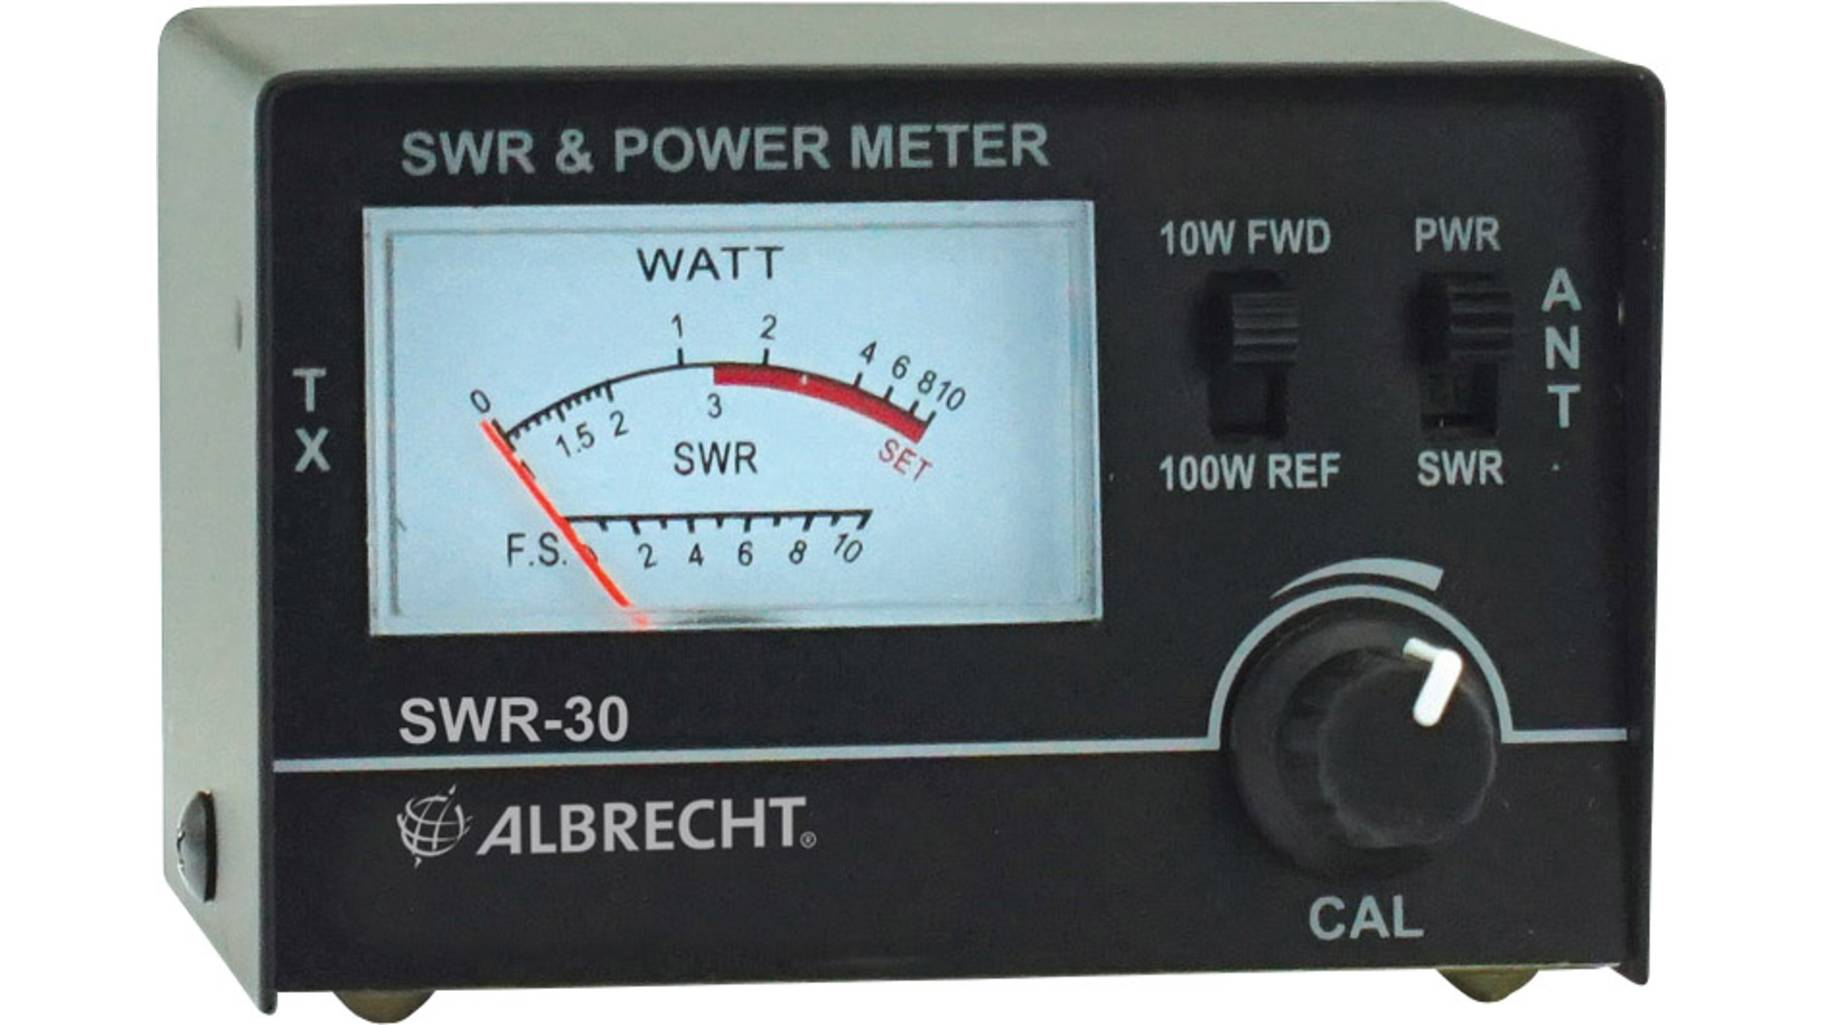
\includegraphics[width=0.85\textwidth]{foto/144}
    \caption{\scriptsize Ein SWR-Meter zur Messung bis maximal \qty{100}{\watt}}
    \label{e_swr_meter_geraet}
\end{figure}

   \end{column}
\end{columns}

\end{frame}

\begin{frame}
\only<1>{
\begin{QQuestion}{EI401}{Ein Stehwellenmessgerät wird eingesetzt bei Sendern zur Messung~...}{der Bandbreite.}
{der Oberwellenausgangsleistung.}
{der Antennenanpassung.}
{des Wirkungsgrades.}
\end{QQuestion}

}
\only<2>{
\begin{QQuestion}{EI401}{Ein Stehwellenmessgerät wird eingesetzt bei Sendern zur Messung~...}{der Bandbreite.}
{der Oberwellenausgangsleistung.}
{\textbf{\textcolor{DARCgreen}{der Antennenanpassung.}}}
{des Wirkungsgrades.}
\end{QQuestion}

}
\end{frame}

\begin{frame}
\only<1>{
\begin{QQuestion}{EI402}{Mit welchem Instrument kann die Anpassung zwischen einem UHF-Sender und der Speiseleitung zur Antenne angezeigt werden?}{Interferometer}
{Universalmessgerät mit Widerstandsanzeige}
{SWR-Meter}
{Anpassungsübertrager}
\end{QQuestion}

}
\only<2>{
\begin{QQuestion}{EI402}{Mit welchem Instrument kann die Anpassung zwischen einem UHF-Sender und der Speiseleitung zur Antenne angezeigt werden?}{Interferometer}
{Universalmessgerät mit Widerstandsanzeige}
{\textbf{\textcolor{DARCgreen}{SWR-Meter}}}
{Anpassungsübertrager}
\end{QQuestion}

}
\end{frame}

\begin{frame}
\only<1>{
\begin{QQuestion}{EI403}{Wie misst man das Stehwellenverhältnis im Sendebetrieb? Man misst es~...}{durch Spannungsmessung am Anfang und am Ende der Speiseleitung.}
{mit einem Absorptionswellenmesser.}
{durch Strommessung am Anfang und am Ende der Speiseleitung.}
{mit einer SWR-Messbrücke.}
\end{QQuestion}

}
\only<2>{
\begin{QQuestion}{EI403}{Wie misst man das Stehwellenverhältnis im Sendebetrieb? Man misst es~...}{durch Spannungsmessung am Anfang und am Ende der Speiseleitung.}
{mit einem Absorptionswellenmesser.}
{durch Strommessung am Anfang und am Ende der Speiseleitung.}
{\textbf{\textcolor{DARCgreen}{mit einer SWR-Messbrücke.}}}
\end{QQuestion}

}
\end{frame}

\begin{frame}
\begin{columns}
    \begin{column}{0.48\textwidth}
    \begin{itemize}
  \item Messung der Antennenanpassung: So nah wie möglich an die Antenne, um Veränderungen der Speiseleitung auszuschließen
  \item Messung der gesamten Anlage: So nah wie möglich hinter dem Sender
  \end{itemize}

    \end{column}
   \begin{column}{0.48\textwidth}
       
\begin{figure}
    \DARCimage{0.85\linewidth}{670include}
    \caption{\scriptsize Prinzip der Messung eines SWR-Meters}
    \label{e_swr_meter_messung}
\end{figure}


   \end{column}
\end{columns}

\end{frame}

\begin{frame}
\only<1>{
\begin{QQuestion}{EI404}{An welcher Stelle muss ein SWR-Meter eingeschleift werden, um möglichst genaue Aussagen über die Antenne machen zu können? Das SWR-Meter muss eingeschleift werden zwischen~...}{Zwischen Anpassgerät und Antennenkabel.}
{Senderausgang und Antennenkabel.}
{Antennenkabel und Antenne.}
{Senderausgang und Antennenanpassgerät.}
\end{QQuestion}

}
\only<2>{
\begin{QQuestion}{EI404}{An welcher Stelle muss ein SWR-Meter eingeschleift werden, um möglichst genaue Aussagen über die Antenne machen zu können? Das SWR-Meter muss eingeschleift werden zwischen~...}{Zwischen Anpassgerät und Antennenkabel.}
{Senderausgang und Antennenkabel.}
{\textbf{\textcolor{DARCgreen}{Antennenkabel und Antenne.}}}
{Senderausgang und Antennenanpassgerät.}
\end{QQuestion}

}
\end{frame}

\begin{frame}
\only<1>{
\begin{PQuestion}{EI405}{An welchem Punkt sollte das Stehwellenmessgerät eingeschleift werden, um zu prüfen, ob die Antennenanlage gut an den Sender angepasst ist? }{Punkt 4}
{Punkt 2}
{Punkt 3}
{Punkt 1}
{\DARCimage{1.0\linewidth}{105include}}\end{PQuestion}

}
\only<2>{
\begin{PQuestion}{EI405}{An welchem Punkt sollte das Stehwellenmessgerät eingeschleift werden, um zu prüfen, ob die Antennenanlage gut an den Sender angepasst ist? }{Punkt 4}
{Punkt 2}
{Punkt 3}
{\textbf{\textcolor{DARCgreen}{Punkt 1}}}
{\DARCimage{1.0\linewidth}{105include}}\end{PQuestion}

}
\end{frame}%ENDCONTENT
